\documentclass{beamer}
\usepackage[utf8]{inputenc}

\usetheme{Madrid}
\usecolortheme{default}
\usepackage{amsmath,amssymb,amsfonts,amsthm}
\usepackage{txfonts}
\usepackage{tkz-euclide}
\usepackage{listings}
\usepackage{adjustbox}
\usepackage{array}
\usepackage{tabularx}
\usepackage{gvv}
\usepackage{lmodern}
\usepackage{circuitikz}
\usepackage{tikz}
\usepackage{graphicx}

\setbeamertemplate{page number in head/foot}[totalframenumber]

\usepackage{tcolorbox}
\tcbuselibrary{minted,breakable,xparse,skins}



\definecolor{bg}{gray}{0.95}
\DeclareTCBListing{mintedbox}{O{}m!O{}}{%
  breakable=true,
  listing engine=minted,
  listing only,
  minted language=#2,
  minted style=default,
  minted options={%
    linenos,
    gobble=0,
    breaklines=true,
    breakafter=,,
    fontsize=\small,
    numbersep=8pt,
    #1},
  boxsep=0pt,
  left skip=0pt,
  right skip=0pt,
  left=25pt,
  right=0pt,
  top=3pt,
  bottom=3pt,
  arc=5pt,
  leftrule=0pt,
  rightrule=0pt,
  bottomrule=2pt,
  toprule=2pt,
  colback=bg,
  colframe=orange!70,
  enhanced,
  overlay={%
    \begin{tcbclipinterior}
    \fill[orange!20!white] (frame.south west) rectangle ([xshift=20pt]frame.north west);
    \end{tcbclipinterior}},
  #3,
}
\lstset{
    language=C,
    basicstyle=\ttfamily\small,
    keywordstyle=\color{blue},
    stringstyle=\color{orange},
    commentstyle=\color{green!60!black},
    numbers=left,
    numberstyle=\tiny\color{gray},
    breaklines=true,
    showstringspaces=false,
}
%------------------------------------------------------------

\title
{5.11.2}
\date{September 16, 2025}
\author 
{AI25BTECH11003 - Bhavesh Gaikwad}



\begin{document}


\frame{\titlepage}
\begin{frame}{Question}
Determine the current in each branch of the network shown in Fig.1
\begin{figure}
    \centering
    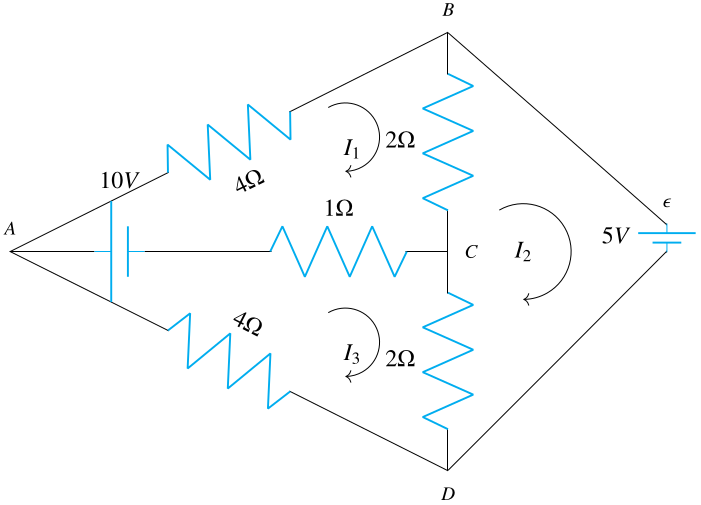
\includegraphics[width=0.75\columnwidth]{figs/figQ.png}
    \caption{Fig.1}
    \label{fig:figs/fig1.png}
\end{figure}
\end{frame}


\begin{frame}[fragile]
    \frametitle{Theoretical Solution}
 Using mesh current analysis with Kirchhoff's Voltage Law (KVL) to solve the question.\\


Applying KVL to the loop ABCA,
\begin{equation}
-7I_1 + 2I_2 + I_3 = -10
\end{equation}


Applying KVL to the loop CBDC,
\begin{equation}
2I_1 - 4I_4 + 2I_3 = -5
\end{equation}

Applying KVL to the loop ACDA,
\begin{equation}
-I_1 - 2I_2 + 7I_3 = 10    
\end{equation}

Therefore, the Three equations are: 
$$ -7I_1 + 2I_2 + I_3 = -10$$
$$2I_1 - 4I_4 + 2I_3 = -5$$
$$-I_1 - 2I_2 + 7I_3 = 10$$\\
\end{frame}


\begin{frame}[fragile]
    \frametitle{Theoretical Solution}
 Let $\vec{M} = \myvec{-7 & 2 & 1 \\ 2 & -4 & 2 \\ -1 & -2 & 7}$ and $\vec{x} = \myvec{I_1 \\ I_2 \\ I_3}$ and $\vec{T} = \myvec{-10 \\ -5 \\ 10}$\\\\

\begin{equation}
    \therefore \, \vec{M}\vec{x}=\vec{T}
\end{equation}

\begin{center}
OR    
\end{center}

\begin{equation}
    \myvec{-7 & 2 & 1 \\ 2 & -4 & 2 \\ -1 & -2 & 7}\vec{x} = \myvec{-10 \\ -5 \\ 10}
\end{equation}

The Augmented Matrix:
\begin{equation}
\left(
\begin{array}{ccc|c}
     -7 & 2 & 1 & -10  \\
     2 & -4 & 2 & -5 \\
     -1 & -2 & 7 & 10 
\end{array}
\right)
\end{equation}
\end{frame}


\begin{frame}[fragile]
    \frametitle{Theoretical Solution}
Row Transformation-1: $R_3 \rightarrow R_3 + R_1$
\begin{equation}
\left(
\begin{array}{ccc|c}
     -7 & 2 & 1 & -10  \\
     2 & -4 & 2 & -5 \\
     -8 & 0 & 8 & 0 
\end{array}
\right)
\end{equation}

Row Transformation-2: $R_2 \rightarrow R_2 + \frac{R_3}{4}$
\begin{equation}
\left(
\begin{array}{ccc|c}
     -7 & 2 & 1 & -10  \\
     0 & -4 & 4 & -5 \\
     -8 & 0 & 8 & 0 
\end{array}
\right)
\end{equation}

Row Transformation-3: $R_3 \rightarrow R_3 - \frac{8R_1}{7} - \frac{4R_1}{7}$
\begin{equation}
\left(
\begin{array}{ccc|c}
     -7 & 2 & 1 & -10  \\
     0 & -4 & 4 & -5 \\
     0 & 0 & 32/7 & -60/7 
\end{array}
\right)
\end{equation}
\end{frame}


\begin{frame}[fragile]
    \frametitle{Theoretical Solution}
 \bigskip

\begin{equation}
    \myvec{-7 &  2 & 1 \\ 0 & -4 & 4 \\ 0 & 0 & 32/7 }\myvec{I_1 \\ I_2 \\ I_3} = \myvec{-10 \\ -5 \\ -60/7 }
\end{equation}

\bigskip

\begin{equation}
\boxed{\therefore I_1 = 55/56 A, \, I_2 = 5/8 A, \, I_3 = 15/8}
\end{equation}
\end{frame}


\end{document}